\documentclass[11pt]{beamer}
\usetheme{Copenhagen}
\usepackage[utf8]{inputenc}
\usepackage[english]{babel}
\usepackage{amsmath}
\usepackage{amsfonts}
\usepackage{amssymb}
\usepackage{graphicx}
\usepackage{caption}
\usepackage{subcaption}
\DeclareMathOperator{\argmin}{\mathrm{arg\, min}}
\author{Onofre Martorell, Lidia Talavera}
\title{Poisson Editing}
%\setbeamercovered{transparent} 
%\setbeamertemplate{navigation symbols}{} 
%\logo{} 
%\institute{} 
%\date{} 
%\subject{} 
\begin{document}

\begin{frame}
\titlepage
\end{frame}

%\begin{frame}
%\tableofcontents
%\end{frame}

\begin{frame}{Introduction}
\begin{block}{Goal}
We want to copy an area of an image using seamless cloning.
\end{block}

An example of the procedure to apply:

\begin{figure}
    \centering
    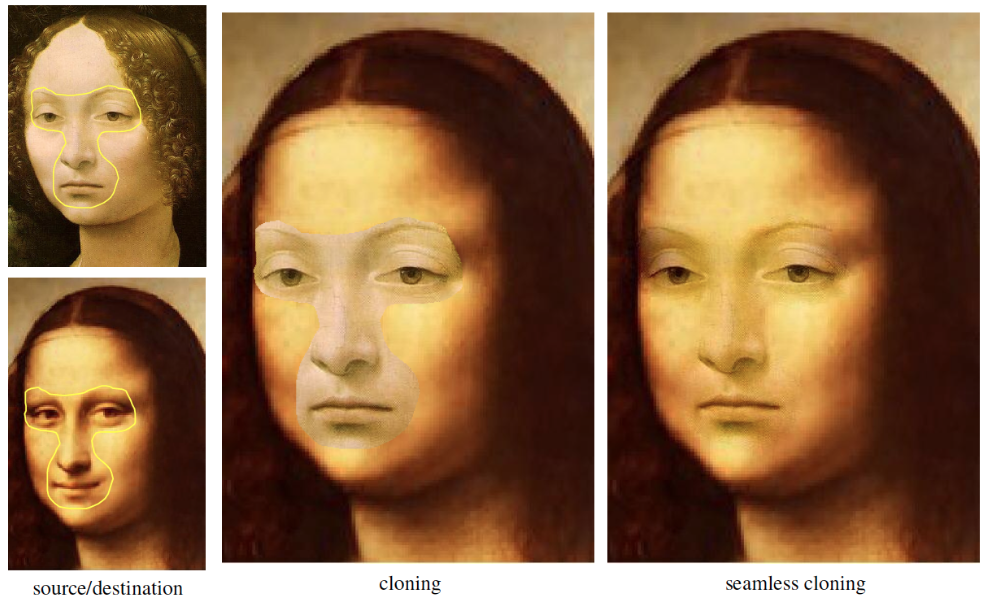
\includegraphics[width=80mm]{Example.png}
\end{figure}
\end{frame}

\begin{frame}{Seamless cloning}
Seamless cloning will be applied through the implementation of the importing gradients method. Let $f^{*}$ be the destination image, $f$ the source image that contains the region we want to clone,  $S \subset \mathbb{R}^{2}$ the domain of the image, $\Omega \subset  S$ a closed subset which will be cloned from $f$ to $f^{*}$  and $\overrightarrow{v}$ the guidance field of vectors defined over $\Omega$.\newline

To solve the problem we have used the next functional over each channel of the image:
\begin{equation}
\min_{f}\int_{\Omega }\left | \nabla f-\overrightarrow{v} \right |^{2},
\label{eq:functional}
\end{equation}

with $f_{\mid \delta \Omega}=f_{\mid \delta \Omega}^{*}$, \newline
\end{frame}

\begin{frame}
The solution of \ref{eq:functional}  is the unique solution of the following Poisson equation with Dirichlet boundary conditions:

\begin{equation}
\left\{\begin{matrix}
 \Delta f=div \overrightarrow{v} & \text{on } & \Omega\\ 
 f=f^{*}& \text{in }\partial\Omega
\end{matrix}\right.
\label{eq:Poisson_general}
\end{equation}

We are using importing gradients, which means that the guidance field $\overrightarrow{v}$ is a gradient field taken directly from a source image. Denoting
by $g$ the source image, this is
$$\overrightarrow{v} = \nabla g.$$

Replacing this in \ref{eq:Poisson_general}, we get
\begin{equation}
\left\{\begin{matrix}
 \Delta f=\Delta g & \text{on } & \Omega\\ 
 f=f^{*}& \text{in }\partial\Omega
\end{matrix}\right.
\end{equation}
%_{\mid \partial \Omega}
%_{\mid \partial \Omega}

\end{frame}

\begin{frame}{Implementation}
In the first week we implemented a numerical method to solve
$$\left\lbrace
\begin{array}{l l}

\Delta f = 0& \text{in }\Omega \\
f = f^* & \text{in }\partial\Omega,

\end{array}\right.
$$
which is a particular case of the method that we need to implement this week. 

What we have done is the following: we have taken the code of the previous week and we have changed it in order to detect if there is a variable containing the discretization of $\nabla g$ for each point of the image. If this variable exists, it computes $\Delta f = \Delta g$; otherwise it computes $\Delta f = 0$.
\end{frame}






\begin{frame}{Results}
We have applied our algorithm to the given images, which goal was to clone the mouth and the eyes of the girl on the left to the girl on the right.
\begin{figure}
    \centering
    \begin{subfigure}[b]{0.36\textwidth}
        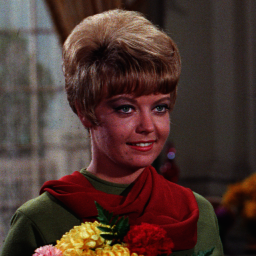
\includegraphics[width=\textwidth]{girl}

    \end{subfigure}
    ~ 
        \begin{subfigure}[b]{0.4\textwidth}
        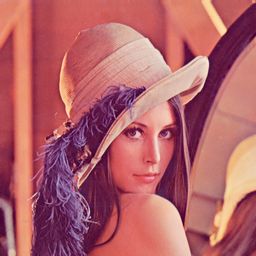
\includegraphics[width=\textwidth]{lena}

    \end{subfigure}

\end{figure}
\end{frame}

\begin{frame}{Results}
This is the results obtained:
\begin{figure}
    \centering
    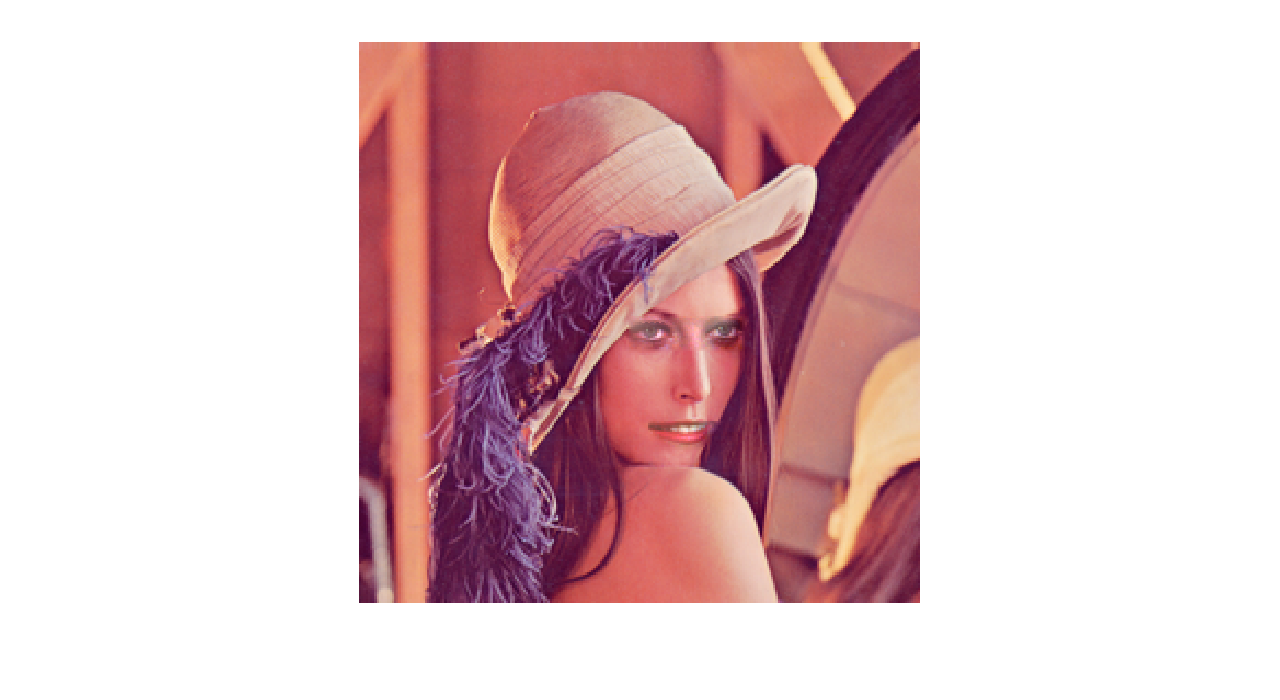
\includegraphics[width=80mm]{lena_result}
\end{figure}
\end{frame}

\begin{frame}{Results}
After solving the problem with the given images, we have tried the method with our own images. The steps done for computing the Poisson editing are the following ones:
\begin{enumerate}
    \item Choose the images to copy.
    \item Crop the source images in order to get the regions to clone.
    \item Using Matlab, make a binary mask of each region.
    \item Remove manually from the mask the points not belonging to the region.
    \item Copy each mask separately to the destination image and create the mask.
    \item Run the code with each cloning region.
\end{enumerate}
\end{frame}

\begin{frame}{Results}
Firs example: cloning the thunderbolt in the other image
\begin{figure}
    \centering
    \begin{subfigure}[b]{0.5\textwidth}
        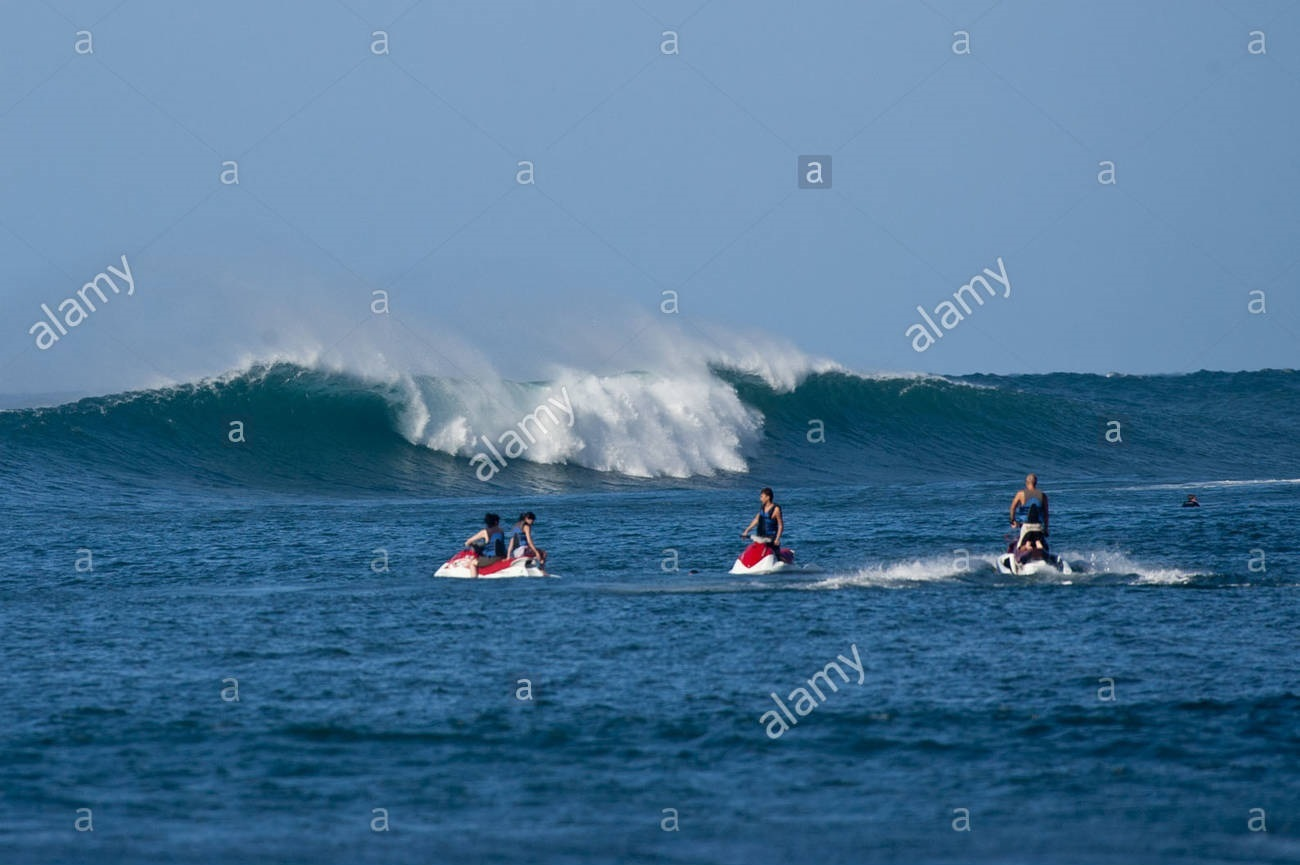
\includegraphics[width=\textwidth]{Mar_motos}

    \end{subfigure}
    ~ 
        \begin{subfigure}[b]{0.3\textwidth}
        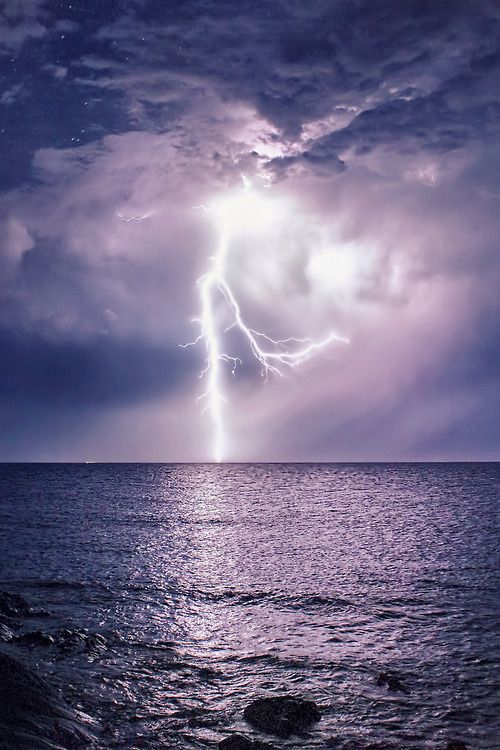
\includegraphics[width=\textwidth]{Thunderbolt}

    \end{subfigure}

\end{figure}
\end{frame}

\begin{frame}{Results}
\begin{figure}
    \centering
    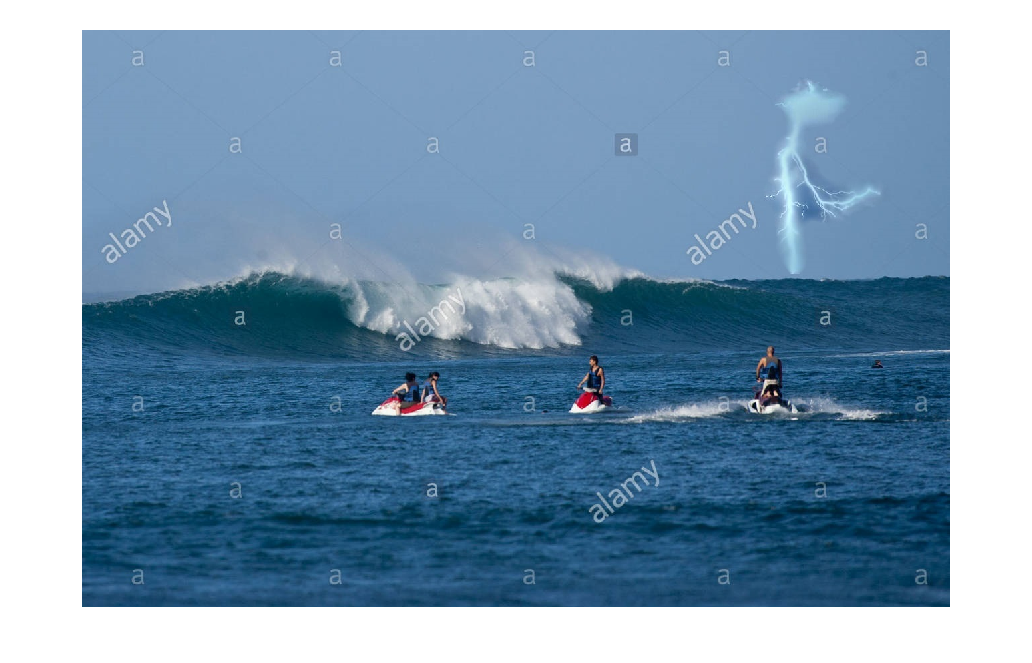
\includegraphics[width=90mm]{Mar_motos_result}
\end{figure}
\end{frame}

\begin{frame}{Results}
Second example: cloning the dog amd the people in the image of the sea
\begin{figure}
    \centering
    \begin{subfigure}[b]{0.36\textwidth}
        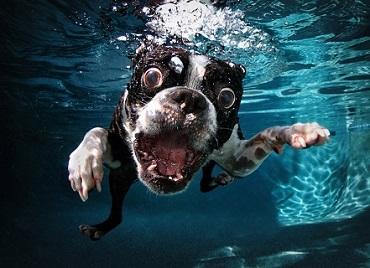
\includegraphics[width=\textwidth]{dog}

    \end{subfigure}
    ~ 
        \begin{subfigure}[b]{0.4\textwidth}
        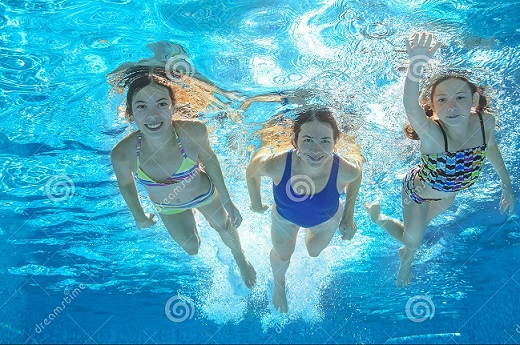
\includegraphics[width=\textwidth]{family_original}

    \end{subfigure}
    
     ~ 
        \begin{subfigure}[b]{0.35\textwidth}
        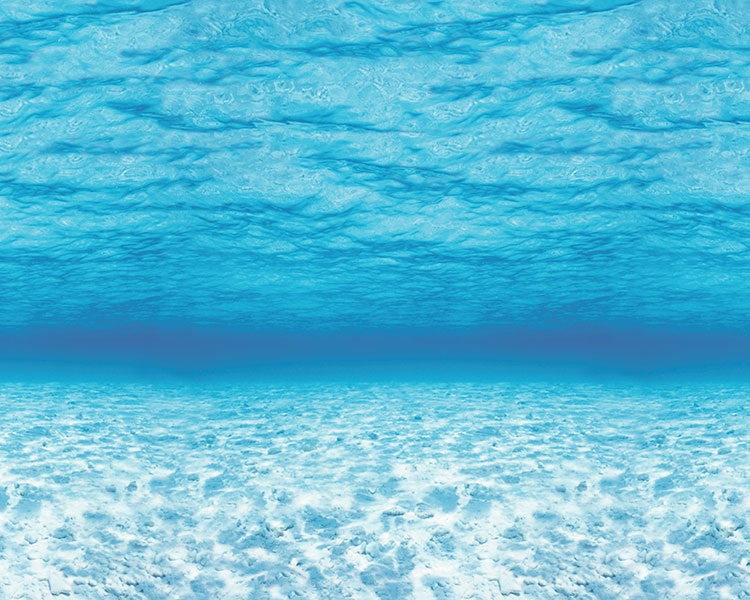
\includegraphics[width=\textwidth]{the_sea}

    \end{subfigure}

\end{figure}
\end{frame}

\begin{frame}{Results}
This is the results obtained:
\begin{figure}
    \centering
    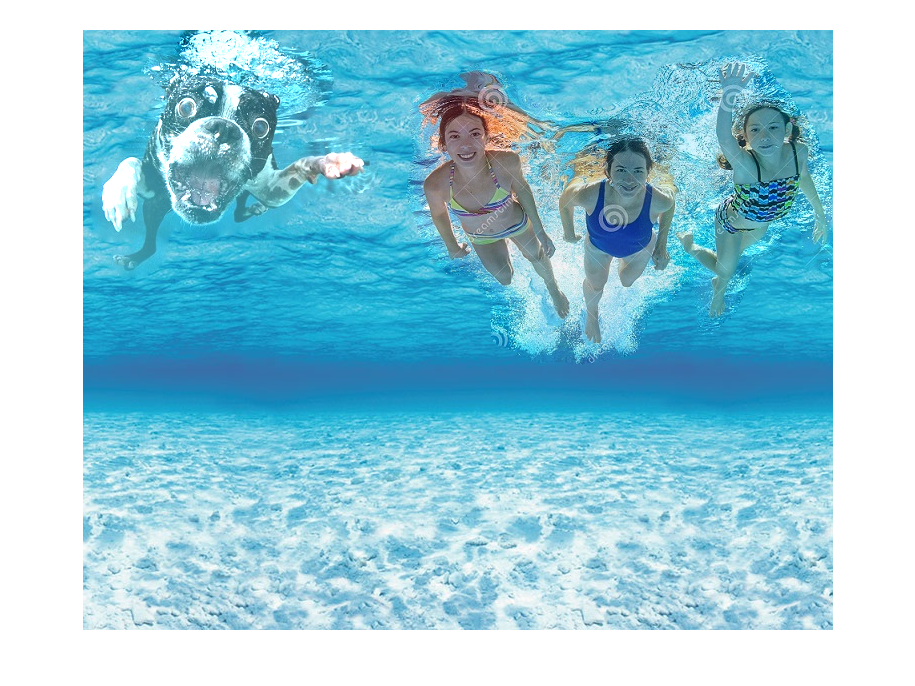
\includegraphics[width=80mm]{The_sea_modified}
\end{figure}
\end{frame}


\begin{frame}{Conclusions}
\begin{itemize}
    \item The method has been easy to implement, because we have reused code from previous weeks.
    \item The most challenging part of using our images was to create the masks correctly.
    \item The results can be improved using mixing gradients instead of importing gradients.
\end{itemize}    
\end{frame}

\end{document}